\section{Auswertung}
\label{sec:Auswertung}

\subsection{Überprüfung der Stabilitätsbedingung} \label{sec:stabilitaet}
Wie in \autoref{sec:Durchführung} beschrieben, 
wird für zum Vermessen der Stabilität eine Resonator-Konfiguration verwendet,
anhand derer man die Stabilitätsbedingung überprüfen kann.
Hierbei wird in \autoref{fig:plot1} für eine konkav-konkav-Konfiguration mit einem Krümmungsradius von $r = \qty{1400}{mm}$ der Photostrom in Abhängigkeit von drei Resonatorlängen gemessen
und mit dem theoretischen Verlauf verglichen.
\begin{figure}
    \centering
    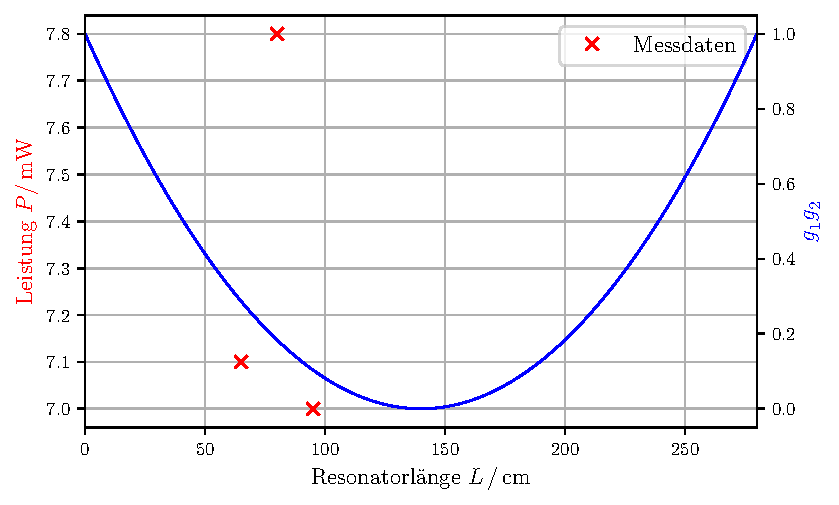
\includegraphics[width=0.8\linewidth]{plot1.pdf}
    \caption{Die Messdaten sowie die Ausgleichsrechnung.}
    \label{fig:plot1}
\end{figure}


\subsection{Beobeachten der TEM-Moden} \label{sec:moden}
Zur Untersuchung der $\text{TEM}_{00}$- und $\text{TEM}_{01}$-Mode wird mithiilfe einer Streulinse
der Laser auf die messende Photodiode gestreut und die Intensität entlang der optischen Achse vermessen.
Die Messdaten und die dazugehörige Regression mittels den Formel
\begin{align}\label{eq:gauss}
    & I_{00} \: \sim \: {\abs{E_{00}}}^2 \: \sim \: a_{00} \cdot           \exp{\left(-\frac{{(x-x_{0_{00}})^2}}{b_{00}}\right)} \quad \text{und} \\
    & I_{01} \: \sim \: {\abs{E_{01}}}^2 \: \sim \: a_{01} \cdot x^2 \cdot \exp{\left(-\frac{{(x-x_{0_{01}})^2}}{b_{01}}\right)} \, .
\end{align}
ergeben mit den Parametern
\begin{align}
    & a_{00} = \qty{7.76(7)}{\micro\ampere} \, , \, b_{00} = \qty{14.7(8)}{} \, , \, x_{0_{00}} = \qty{60.3(1.8)}{} \, , \\
    & a_{01} = \qty{0.031(0.007)}{\micro\ampere} \, , \, b_{01} = \qty{2.1(7)}{} \, , \, x_{0_{01}} = \qty{86(14.0)}{} \, ,
\end{align}
die in \autoref{fig:moden} stehenden Plots.
\begin{figure}[H]
    \centering
    
    \begin{subfigure}{0.7\columnwidth}
        \centering
        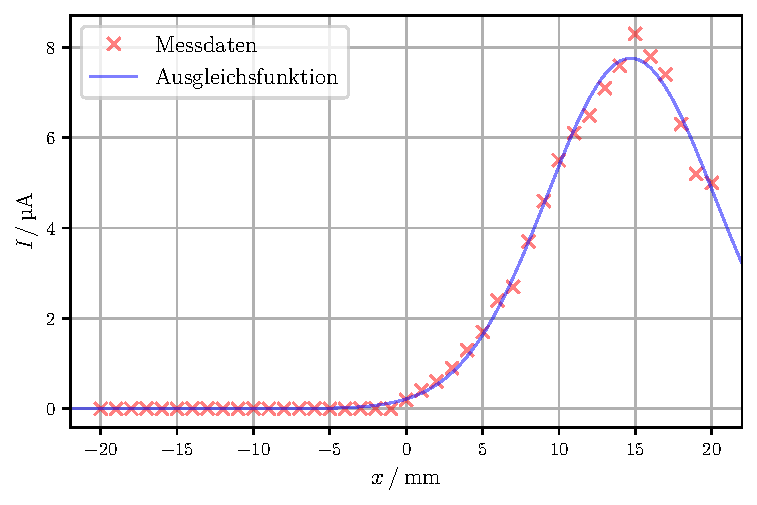
\includegraphics[width=\textwidth]{plot2_00.pdf}
        \caption{Intensitätsverteilung für die $\text{TEM}_{00}$-Mode.}
        \label{fig:tem00}
    \end{subfigure}\hfill

    \begin{subfigure}{0.7\columnwidth}
        \centering
        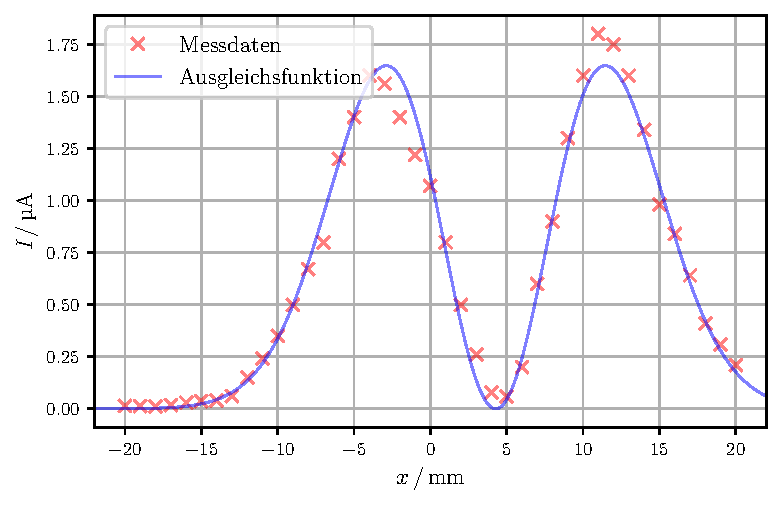
\includegraphics[width=\textwidth]{plot2_01.pdf}
        \caption{Intensitätsverteilung für die $\text{TEM}_{01}$-Mode.}
        \label{fig:tem01}
    \end{subfigure}
  
    \caption{Die Intensitätsverteilungen der zu untersuchenden Moden.}
    \label{fig:moden}
  
\end{figure}


\subsection{Bestimmung der Polarisation} \label{sec:polarisation}
Die Intensität folgt der Gleichung
\begin{equation}
    I(\varphi)=I_0 \cdot \cos ^2 \left(\varphi+\varphi_0\right) \, .
\end{equation}
Die in \autoref{fig:plot3} abgebildete Fit an die gemessenen Intensitäten in Abhängigkeit des Polarisationswinkel ergibt die Parameter
\begin{align*}
    I_0 = \qty{4.1(9)}{\micro\ampere} \quad \text{und} \quad \varphi_0 = \qty{2.23(17)}{\degree} \, .
\end{align*}

\begin{figure}
    \centering
    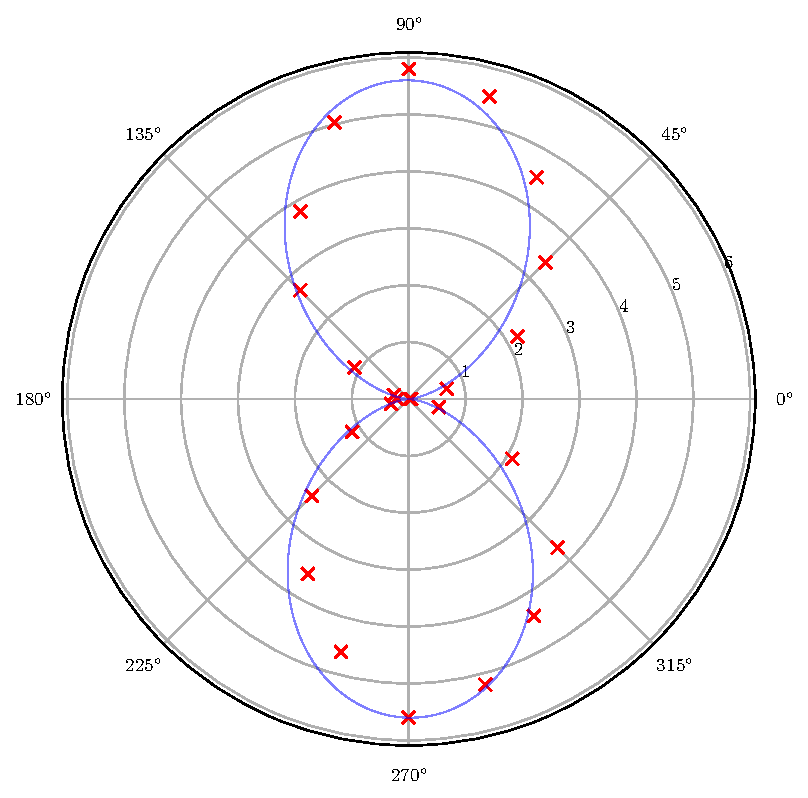
\includegraphics[width=0.8\linewidth]{plot3.pdf}
    \caption{Der Polarplot der Intensitäten und deren Regression.}
    \label{fig:plot3}
\end{figure}


\subsection{Frequenzspektrum des Lasers} \label{sec:spektrum}
Im Zusammenhang mit \autoref{sec:stabilitaet} werden für die drei Resonatorlängen die Fourierspektren gemessen,
diese sind in \autoref{tab:spektren} dargestellt.
\begin{table}
    \centering
    \caption{Die gemessenen Spektren für die drei Resonatorlängen.}
    \label{tab:spektren}
    \begin{tabular}{c c c c c c c c}
        \toprule
        $L \, / \, cm$ & $\nu_1$ & $\nu_2$ & $\nu_3$ & $\nu_4$ & $\nu_5$ & $\nu_6$ & $\nu_7$ \\
        \midrule
           65 &  248 &  493 &  738 &  983 &       &        &        \\
           80 &  191 &  383 &  570 &  761 & 953 & 1140 &        \\
           95 &  101 &  318 &  980 &  638 & 795 &  956 & 1140 \\
        \bottomrule
    \end{tabular}
\end{table}


\subsection{Bestimmung der Wellenlänge} \label{sec:lambda}
Die aufgenommenen Abstände der Maxima $n$ zum Hauptmaximum $n = 0$ der Gitter mit den Gitterkonstanten $g_1 = 80 \text{Linien}/\mathrm{cm}$ (Abstand $d_1 = \qty{41,5}{cm}$) und
$g_2 = 100 \text{Linien}/\mathrm{cm}$ (Abstand $d_2 = \qty{30}{cm}$) sind in \autoref{tab:abstaende} dargestellt.
\begin{table}
    \centering
    \caption{Abstände der Maxima zum Hauptmaximum für die zwei verwendeten Gitter.}
    \label{tab:abstaende}
    \begin{tabular}{c c c}
        \toprule
           &  80 Linien $/ \, \mathrm{cm}$ &  100 Linien $/ \, \mathrm{cm}$ \\
         n &  $x \, / \, \mathrm{cm}$ &  $x \, / \, \mathrm{cm}$ \\
        \midrule
         1 &     2,2 &       2,0 \\
        -1 &     2,2 &       2,0 \\
         2 &     4,3 &       3,9 \\
        -2 &     4,3 &       4,0 \\
         3 &     6,3 &       5,9 \\
        -3 &     6,6 &       6,0 \\
        \bottomrule
    \end{tabular}
\end{table}
Dabei beschreibt die Ordnung $n>0$ die auftretenden Maxima zur rechten Seite
senkrecht zur optischen Achse und $n<0$ die Maxima zur linken Seite.

Mithilfe der Formel
\begin{equation}
    \lambda=\frac{g \cdot \sin \alpha_n}{n} = \frac{x_n \cdot g}{n \cdot \sqrt{d^2+x_n^2}}
\end{equation} 
werden die Wellenlängenberechnungen an den einzelnen Intensitätsmaxima durchgeführt. 
Die daraus resultierenden Werte für $\lambda$ ergeben nach einer Mittelung
\begin{align*}
    \bar{\lambda_{80}} = \qty{655.06}{\nano\meter} \quad \text{und} \\
    \bar{\lambda_{100}} = \qty{666.57}{\nano\meter} \, .
\end{align*}
